\documentclass[11pt,fleqn]{exam}
\usepackage[utf8]{inputenc}

\usepackage[margin=1in]{geometry}
\usepackage{amsmath,amssymb}
\usepackage{multicol}
\usepackage{float}

\hyphenation{
  chro-no-ampe-ro-met-ric
  ber-dia-me-ter
  de-ngan
  me-nem-pati
  mic-ro-graphs}


\usepackage{graphicx}
\renewcommand{\figurename}{Gambar.}
\usepackage[margin=1.5cm]{caption}

\newcommand{\class}{OLIMPIADE ASTRONOMI}
\newcommand{\term}{Tingkat Provinsi - 2014}
\newcommand{\examnum}{OSP Astronomi 2014}
\newcommand{\examdate}{1/1/2014}
\newcommand{\timelimit}{60 Minutes}

\pagestyle{head}
\firstpageheader{}{}{}
\runningheader{\examnum}{}{Halaman \thepage\ dari \numpages}
\runningheadrule


\begin{document}

\noindent
\begin{tabular*}{\textwidth}{l @{\extracolsep{\fill}} r @{\extracolsep{6pt}} l}
\textbf{\class} \\% & \textbf{Name:} & \makebox[2in]{\hrulefill}\\
\textbf{\term}  %&&\\
%\textbf{\examnum} &&\\
%\textbf{\examdate} &&\\
%\textbf{Time Limit: \timelimit} & Teaching Assistant & \makebox[2in]{\hrulefill}
\end{tabular*}\\
\rule[2ex]{\textwidth}{2pt}

\noindent
\begin{tabular}{ll}
Copyright (c) 2014 & Ridlo W. Wibowo (ridlo.w.wibowo@gmail.com)\\
                   & Sulistiyowati (sulis.astro08@gmail.com)
\end{tabular}

\vspace{0.3cm}
\noindent
Solusi ini dibuat tanpa jaminan kesesuaian dengan solusi resmi dari juri olimpiade sains bidang Astronomi. Pengguna boleh menyebarluaskan dan/atau memodifikasi solusi ini dengan mencantumkan sumber asli. Hak cipta soal ada pada Kemendiknas dan dilindungi undang-undang.

\vspace{0.4cm}
\noindent
\rule[2ex]{\textwidth}{1.5pt}

\textbf{Soal Pilihan Berganda}

\begin{questions}
\question Apakah yang dimaksud dengan luminositas Matahari?
\begin{choices}
\choice Besarnya energi yang dipancarkan oleh Matahari
\choice Besarnya energi Matahari yang diterima di permukaan Bumi
\choice Kecerlangan Matahari yang diukur pada jarak tertentu
\choice Terang sebenarnya Matahari yang sampai ke Bumi
\choice Daya Matahari yang diterima di Bumi per satuan luas per satuan waktu
\end{choices}

Jawaban: A

Luminositas Matahari menyatakan jumlah energi total yang dipancarkan Matahari per satuan waktu.\\

\question Secara spektroskopi, astronom mendeteksi kehadiran medan magnet pada objek-objek astronomi melalui
\begin{choices}
\choice efek Zeeman
\choice terowongan kuantum
\choice keberadaan garis-garis Balmer
\choice efek polarisasi
\choice bentuk kurva benda hitam
\end{choices}

Jawaban: A

Efek Zeeman adalah efek pemisahan sebuah garis spektrum menjadi beberapa komponen disebabkan oleh adanya medan magnet. Seperti halnya percobaan yang membuktikan bahwa orbital $p$ memiliki 3 sub-orbital (lihat garis tunggal yang terlihat terpisah menjadi 3 garis seperti pada gambar dibawah ini).

Contoh:
\begin{figure}[H]
\centering
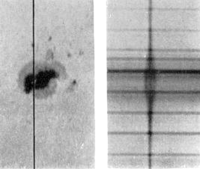
\includegraphics[width=0.175\textwidth]{Sun_zeeman.png}
\caption{Efek Zeeman diamati saat memeriksa spektrum bintik Matahari, menandakan aktifitas magnetik yang kuat. Hale - G.E. Hale, F. Ellerman, S.B. Nicholson, and A.H. Joy in ApJ Vol. 49, pps. 153-178.}
\end{figure}

\question Sebuah bintang memiliki jejari 2000 km dan temperatur 10000 K. Jika jarak bintang ini 10 parsek maka, maka bintang
\begin{choices}
\choice sulit diamati dengan mata telanjang karena jaraknya terlalu jauh
\choice sulit diamati dengan mata telanjang karena nilai magnitudonya yang terlalu besar
\choice relatif lebih mudah diamati dengan mata telanjang karena temperaturnya yang tinggi
\choice relatif lebih mudah diamati dengan mata telanjang karena nilai magnitudonya yang besar
\choice tidak dapat disimpulkan apakah dapat diamati dengan mata telanjang atau tidak
\end{choices}

Jawaban: A \& B

Cek dulu pernyataan tersebut. Bandingkan dengan Matahari. Digunakan nilai magnitudo mutlak Matahari 4,8.\\

\begin{eqnarray*}
M-M_{\odot}&=&-2,5\log(\dfrac{L}{L_{\odot}})\\
&=&-2,5\log(\dfrac{4\pi R^{2}\sigma T^{4}}{4\pi R_{\odot}^{2}\sigma T_{\odot}^{4}})\\
M &=&15,15
\end{eqnarray*}

Pada jarak 10 parsek, magnitudo mutlak benda = magnitudo semunya, sehingga magnitudo hasil penghitungan di sini (15,15) berperan sebagai magnitudo semu yang teramati oleh mata manusia. Rata-rata mata manusia bisa mengamati objek langit hingga magnitudo 6, magnitudo ini terlalu redup (dengan kata lain terlalu besar) untuk bisa diamati dengan mata telanjang. Dengan pernyataan ini, jawaban B valid.

Pada jarak 10 parsek, objek ini telalu redup untuk bisa diamati dengan mata telanjang. Namun, objek ini bisa jadi teramati jika jaraknya lebih dekat ke pengamat. Dengan demikian, pernyataan A juga valid.\\


\question Jarak dari pusat Bumi ke sebuah satelit yang bergerak melingkari Bumi dengan periode orbit 150% periode sideris Bulan adalah 
\begin{choices}
\choice $1,02 \times 10^{8}$ meter 
\choice $2,02 \times 10^{8}$ meter
\choice $3,02 \times 10^{8}$ meter
\choice $4,02 \times 10^{8}$ meter
\choice $5,02 \times 10^{8}$ meter
\end{choices}

Jawaban: E

Hukum ketiga Kepler dapat diturunkan dari hukum gravitasi Newton menjadi:\\
\begin{equation*}
\frac{4 \pi^{2} a^{3}}{P^{2}} = GM
\end{equation*}
dalam kasus ini $M$ adalah massa Bumi. Jika kita bandingkan antara satelit dan Bulan dengan jarak rata-rata Bumi-Bulan $a_m = 384400$ km, maka:
\begin{eqnarray*}
\frac{4 \pi^{2} a_{s}^{3}/P_{s}^{2}}{4 \pi^{2} a_{m}^{3}/P_{m}^{2}} &=& \frac{GM_{\oplus}}{GM_{\oplus}}\\
\frac{a_{s}^{3}}{P_{s}^{2}} &=& \frac{a_{m}^{3}}{P_{m}^{2}}\\
a_{s} &=& a_{m}  \sqrt[3]{\left( \frac{P_{s}}{P_{m}}\right)^{2}} \\
a_{s} &=& a_{m}  \sqrt[3]{\left(1.5\right)^{2}} \\
a_{s} &=& 1.31 a_{m}\\
a_{s} &=& 5.02 \times 10^{8} \text{  meter}
\end{eqnarray*}

\question Panjang satu tahun kabisat pada Kalender Matahari Kala Sunda (KMKS) dan Kalender Matahari Gregorian (KMG) adalah 366. Panjang satu tahun basit pada kedua kalender tersebut adalah 365 hari. Aturan tahun kabisat pada KMKS adalah setiap tahun yang habis dibagi 4 dan tidak habis dibagi 128. Aturan tahun kabisat pada KMG adalah setiap tahun kelipatan 100 yang habis dibagi 400, atau setiap tahun bukan kelipatan 100 yang habis dibagi 4. Aturan tahun basit pada kedua kalender tersebut adalah tahun yang tidak memenuhi aturan tahun kabisat. Dengan demikian, dalam kurun waktu 51200 tahun
\begin{choices}
\choice KMG mempunyai 16 tahun kabisat lebih banyak daripada KMKS
\choice KMKS mempunyai 16 tahun kabisat lebih banyak daripada KMG
\choice KMG mempunyai jumlah tahun kabisat sama dengan KMKS
\choice KMG mempunyai 31 tahun kabisat lebih banyak daripada KMKS
\choice KMKS mempunyai 31 tahun kabisat lebih banyak daripada KMG
\end{choices}

Jawaban: A

Jumlah tahun kabisat pada KMKS selama 51200 tahun = $\frac{51200}{4}-\frac{51200}{128}$ = 12400

Jumlah tahun kabisat pada KMG selama 51200 tahun = $\frac{51200}{4}-\frac{51200}{100}\frac{3}{4}$ = 12416\\


\question Jika sabit tipis Bulan tampak sesaat sebelum Matahari terbit, berarti Bulan menuju ke fase
\begin{choices}
\choice Bulan Baru
\choice Seperempat pertama
\choice Purnama
\choice Seperempat akhir
\choice Gembung Bulan
\end{choices}

Jawaban: A

Saat Bulan sabit ``tua'' yaitu Bulan sedang menuju fase Bulan Baru maka ia akan terbit sesaat sebelum Matahari terbit, berada di meredian saat hampir tengah hari, dan akan tenggelam sesaat sebelum Matahari tenggelam. Hal ini dapat dijelaskan dengan sederhana menggunakan diagram fase Bulan seperti di bawah ini. Rotasi Bumi dan revolusi Bulan arah putarnya berlawanan arah jarum jam, sehingga pagi hari adalah bagian bawah gambar Bumi. Terlihat bahwa posisi Bulan Baru adalah searah dengan arah Matahari, oleh karena itu jika dilihat oleh pengamat yang sedang mengalami ``pagi hari'' ia akan terbit hampir bersamaan dengan Matahari terbit.

\begin{figure}[H]
\centering
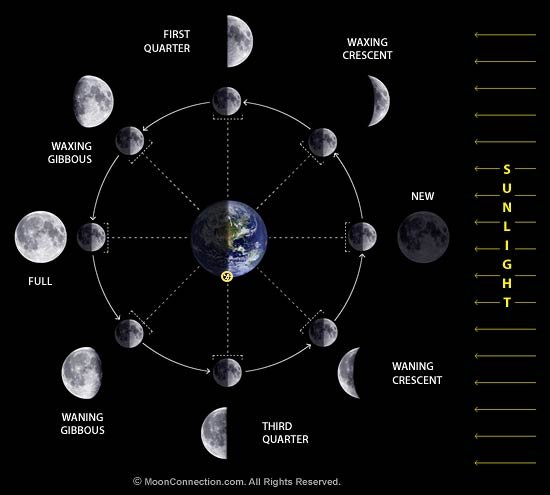
\includegraphics[width=0.5\textwidth]{moon_phases.jpg}
\caption{Diagram fase Bulan. Sumber gambar: MoonConnection.com}
\label{overflow}
\end{figure}


\question Komposisi atom di fotosfer Matahari dapat dipelajari dengan
\begin{choices}
\choice mengamati jumlah bintik Matahari
\choice menerapkan hukum pergeseran Wien dalam spektrum Matahari
\choice menelaah garis absorpsi spektrum Matahari
\choice mengamati Korona pada saat terjadinya Gerhana Matahari Total
\choice mengamati siklus Matahari terus menerus
\end{choices}

Jawaban: C

Tiap-tiap atom memiliki konfigurasi inti atom dan elektron sendiri-sendiri. Tiap elektron menempati lokasi (kulit) dengan tingkat energi yang spesifik, sehingga perpindahan elektron dari satu kulit ke kulit lain pun memerlukan energi yang spesifik pula. Elektron yang naik ke kulit lebih luar (tingkat energi lebih tinggi) akan menyerap energi yang dengan panjang gelombang tertentu yang bersesuaian dengan energi yang diperlukan. Absorpsi energi pada panjang gelombang tertentu oleh elektron-elektron atom tertentu ini dapat diamati pada spektrum bintang.\\


\question Jika Matahari berada pada jarak 4,37 tahun cahaya, apakah Matahari masih dapat kita amati tanpa alat bantu teleskop
\begin{choices}
\choice Tidak, karena jarak Matahari terlalu jauh dari Bumi sehingga sulit diamati hanya dengan mata telanjang
\choice Ya, karena jarak tidak mempengaruhi seberapa besar fluks energi Matahari yang diterima di Bumi
\choice Tidak, karena luminositas Matahari menjadi jauh lebih kecil dibandingkan ketika berada lebih dekat dengan Bumi
\choice Ya, karena magnitudo semunya masih dalam rentang pengamatan mata manusia
\choice Belum bisa diketahui, bergantung temperatur Matahari ketika berada pada jarak yang lebih jauh
\end{choices}

Jawaban: D

Misal menggunakan magnitudo mutlak Matahari = 4.83
\begin{eqnarray*}
m - M &=& -5 + 5 \log d \\
m &=& 4.83 - 5 + 5 \log 1.33675353\\
m &=& 0.46  
\end{eqnarray*}
jelas terlihat, karena $m < 6$.\\


\question Sebuah satelit dengan massa 1000 kg bergerak dalam orbit lingkaran pada ketinggian 400 km dari permukaan Bumi. Kecepatan linear satelit tersebut adalah
\begin{choices}
\choice 7,67 km/s
\choice 7,90 km/s
\choice 10,84 km/s
\choice 11,20 km/s
\choice 31,56 km/s
\end{choices}

Jawaban: A

\begin{eqnarray*}
v_{circ}&=&\sqrt{\dfrac{GM_{\oplus}}{R_{\oplus}+h}}\\
&=&7671,57 \text{  m/s}\\
&=&7,67 \text{  km/s}
\end{eqnarray*}


\question Berikut ini adalah koordinat ekuator dua benda langit pada tanggal 9 April 2014: Mars $\alpha = 13^{j}12^{m}$, $\delta = -5^{\circ}2'$ dan Matahari $\alpha = 1^{j}10^{m}$, $\delta = +7^{\circ}23'$. Dari sebuah pulau kecil dengan lintang geografis $0^{\circ}$, berapa lamakah pada malam itu Mars berada di atas horizon?
\begin{choices}
\choice 12 jam
\choice 14 jam
\choice 2 jam
\choice 6 jam
\choice 7 jam
\end{choices}

Jawaban: A

Bagi pengamat di lintang geografis $0^{\circ}$ semua bintang di langit akan berada di atas horizon yaitu sama $\sim 12$ jam (kecuali bintang yang berada tepat di atas Kutub), sehingga deklinasi dua objek ini bisa dikatakan tidak berpengaruh pada lamanya ia di atas horizon. Pada tanggal 9 April selisih asensiorekta dari dua objek ini adalah $\sim 12$ jam, sehingga saat Matahari tenggelam akan bersamaan dengan terbitnya Mars, maka lama Mars berada di atas horizon saat malam hari itu adalah $\sim 12$ jam.\\


\question Dua bintang berjejari sama masing-masing mempunyai temperatur 6000 K dan 5000 K. Energi yang dihasilkan oleh bintang yang temperaturnya lebih tinggi adalah ... kali lebih besar dari bintang yang temperaturnya lebih rendah.
\begin{choices}
\choice 1,2
\choice 1,4
\choice 1,6
\choice 1,8
\choice 2,1
\end{choices}

Jawaban: E

Dengan menganggap bintang sebagai benda hitam sempurna, berlaku
\begin{eqnarray*}
E \propto T^{4}\\
\dfrac{E_{1}}{E_{2}}&=&\dfrac{T_{1}^{4}}{T_{2}^{4}}\\
&=&2,1
\end{eqnarray*}


\question Dari kurva Planck tiga pemancar benda hitam dengan temperatur masing-masing $T_1 = 12000$ K, $T_2 = 9000$ K, dan $T_3 = 6000$ K, maka perbandingan panjang gelombang intensitas maksimum pemancar adalah
\begin{choices}
\choice $\lambda_2 = 3 \lambda_1/4$, $\lambda_3 = 2\lambda_1$
\choice $\lambda_2 = 4 \lambda_1/3$, $\lambda_3 = \lambda_1/2$
\choice $\lambda_2 = 4 \lambda_1/3$, $\lambda_3 = 2\lambda_1$
\choice $\lambda_2 = 3 \lambda_1/4$, $\lambda_3 = \lambda_1/2$
\choice $\lambda_2 = 2 \lambda_1$, $\lambda_3 = 4\lambda_1/3$
\end{choices}

Jawaban: C

Hukum Wien menyatakan bahwa $\lambda_{max} = 0.002898/T$, atau panjang gelombang pada intensitas maksimum benda hitam berbanding terbalik dengan temperaturnya.\\
$\lambda_2 / \lambda_1 = T_1 / T_2 = 4/3$ \\
$\lambda_3 / \lambda_1 = T_1 / T_3 = 2$\\


\question Venus adalah planet kedua terdekat dari Matahari setelah Merkurius, tetapi temperatur rata-rata permukaannya lebih tinggi dibandingkan dengan Merkurius. Hal ini disebabkan oleh
\begin{choices}
\choice bombardir meteor yang menerus di permukaan Venus
\choice albedo Venus yang sama dengan Merkurius yakni 0,75
\choice $CO_{2}$ pada atmosfer Venus memberikan efek rumah kaca
\choice kerapatan Venus sama dengan kerapatan Bumi yakni 5300 kg/m$^3$
\choice ukuran Venus lebih besar daripada ukuran Merkurius
\end{choices}

Jawaban: C

Venus memiliki atmosfer tebal yang didominasi $CO_2$. $CO_2$ merupakan salah satu gas yang dapat menimbulkan efek rumah kaca. Sebagian energi Matahari yang datang ke Venus terjebak di dalam sehingga mengakibatkan temperatur permukaan Venus tinggi.\\


\question Pesawat rover Pathfinder yang diluncurkan oleh Amerika melakukan pemotretan di permukaan planet Mars, dengan perintah yang dikirim dari Bumi melalui gelombang radio. Perintah diberikan pada pukul 23:05 saat oposisi Mars. Jika proses menerima perintah, mengarahkan kamera, memotret lalu mengirimkan datanya ke Bumi membutuhkan waktu 7 menit, pada pukul berapa stasiun pengendali di Amerika menerima fotonya? Anggap Bumi dan Mars mengelilingi Matahari dalam orbit lingkaran.
\begin{choices}
\choice 23:09
\choice 23:12
\choice 23:16
\choice 23:20
\choice 23:25
\end{choices}

Jawaban: D

Saat oposisi jarak Bumi-Mars = 0.52 SA = 77792000 km\\
Waktu tempuh gelombang elektromagnetik = $\frac{77792000}{3\times 10^5}$ = 259.3 detik = 4.32 menit\\
Total waktu yang dibutuhkan = $4.32 \times 2 + 7 = 15.6$ menit\\
Jika sinyal dipancarkan pukul 23:05 maka dapat diperoleh sinyal balasan pada pukul 23:21\\


\question Agar sebuah teleskop dapat melihat dengan jelas sebuah kawah di Bulan dengan diameter 2 kilometer, maka teleskop itu harus mempunyai daya pisah
\begin{choices}
\choice kurang dari 1,0 detik busur
\choice sekitar 1,2 detik busur
\choice lebih besar dari 1,4 detik busur
\choice 1,6 detik busur
\choice antara 1,5 dan 1,8 detik busur
\end{choices}

Jawaban: A

Tentukan diameter sudut kawah.
\begin{eqnarray*}
\sin \frac{\delta}{2}&=&\dfrac{1}{384400}\\
\delta &=&1,02"
\end{eqnarray*}
Diameter sudut kawah dari Bumi $\approx$ 1,02".\\


\question Jarak terdekat komet P/Halley (periode = 76 tahun) ke Matahari adalah $8.9 \times 10^{10}$ meter. Eksentrisitasnya adalah 
\begin{choices}
\choice 0,567
\choice 0,667
\choice 0,767
\choice 0,867
\choice 0,967
\end{choices}

Jawaban: E

Menggunakan hukum Kepler III seperti pada soal sebelumnya akan diperoleh $a = \sqrt[3]{76^2} = 17.9422$ SA $= 2.684153 \times 10^{12}$ meter.\\
$r_{min} = a(1-e)$, sehingga diperoleh e = 0.967.\\


\question Pilih mana yang BENAR
\begin{choices}
\choice Panjang gelombang dari garis emisi yang dihasilkan oleh sebuah elemen berbeda dari panjang gelombang garis absorpsi yang dihasilkan oleh elemen yang sama.
\choice Energi foton berbanding terbalik dengan panjang gelombang radiasinya.
\choice Energi foton berbanding lurus dengan panjang gelombang radiasinya.
\choice Garis spektrum hidrogen relatif lemah pada Matahari karena Matahari mengandung hidrogen yang lebih sedikit.
\choice Garis Fraunhofer adalah garis emisi dalam spektrum Matahari.
\end{choices}

Jawaban: B

Menurut Planck, satu foton memiliki energi sebesar
\begin{eqnarray*}
E=\dfrac{hc}{\lambda}
\end{eqnarray*}
dengan $\lambda$ menyatakan panjang gelombang.\\


\textbf{Pilihan Ganda Bersyarat}\\
A. jika 1, 2, dan 3 benar\\
B. jika 1 dan 3 benar\\
C. jika 2 dan 4 benar\\
D. jika 4 saja benar\\
E. jika semua benar\\

{%
% changing choice items style locally
\renewcommand*\thechoice{\arabic{choice}} 
%
\question Hingga saat ini, anggota Tata Surya yang diketahui mempunyai medan magnet adalah
\begin{choices}
\choice Bumi
\choice Venus
\choice Jupiter
\choice Mars
\end{choices}

Jawaban: B

Mars dan Venus diketahui memiliki medan magnet yang sangat kecil, diduga ia tidak memiliki inti cair yang bergerak (atau sudah membeku) yang merupakan sumber medan magnet sebuah planet.\\


\question Satelit alami yang saat ini diketahui TIDAK mempunyai atmosfer adalah
\begin{choices}
\choice Bulan
\choice Titan
\choice Phobos
\choice Io
\end{choices}

Jawaban: B

Gravitasi Bulan dan Phobos tidak mampu mengikat gas untuk dijadikan sebagai lapisan atmosfer. Meskipun Titan dan Io gravitasinya tidak jauh berbeda dengan Bulan namun lokasi yang jauh dari Matahari menjadikan suhunya lebih dingin. Suhu yang dingin ini mengakibatkan energi kinetik yang dimiliki gas tidak terlalu besar untuk menjadikannya lepas dari ikatan gravitasi.\\


\question Jika kita menggunakan teropong bintang untuk meneropong objek-objek di permukaan Bumi, akan tampak citranya terbalik. Sesungguhnya ahli optik dapat saja membuatnya tidak terbalik, seperti jika kita menggunakan teropong medan (binokuler). Mengapa teropong bintang tidak dirancang untuk menghasilkan citra tegak? Karena untuk menghasilkan citra tegak 
\begin{choices}
\choice biaya produksi akan lebih tinggi
\choice diperlukan lensa tambahan yaitu lensa pembalik
\choice risiko kehilangan energi cahaya di dalam teropong akan lebih besar
\choice tidak sesuai dengan prinsip-prinsip astronomi
\end{choices}

Jawaban: A

Butuh lensa tambahan untuk membalikkan citra, hal ini akan menambah biaya produksi, risiko kehilangan energi cahaya, serta gangguan lain pada citra. \\
}%


\newpage
\textbf{Soal Essay Pendek}

\question Dari definisi pergeseran merah (\textit{redshift, z}) dan hukum pergeseran Wien akan didapatkan hubungan temperatur dan \textit{redshift}, \textit{T}(\textit{z}). Saat ini temperatur radiasi latar belakang (\textit{Cosmic Microwave Background}, \textit{CMB}) yang teramati adalah sebesar 2,7 K. Berapa temperatur \textit{CMB} pada pergeseran merah \textit{z=}9?

Jawaban:

Hukum Wien menyatakan hubungan antara panjang gelombang dan temperatur sebagai berikut.

\begin{eqnarray*}
\lambda=\dfrac{b}{T}
\end{eqnarray*}

sehingga berlaku

\begin{eqnarray*}
z=\dfrac{\lambda_{obs}-\lambda_e}{\lambda_e}&=&\dfrac{\frac{b}{T_{obs}}-\frac{b}{T_e}}{\frac{b}{T_e}}\\
z&=&\dfrac{T_e}{T{obs}}-1\\
T_e&=&(z+1)T_{obs}\\
T_e&=&27 \text{   K}
\end{eqnarray*}
Temperatur \textit{CMB} pada pergeseran merah \textit{z=}9 adalah 27 K.\\


\question Sebuah asteroid mengorbit Matahari tepat di bidang ekliptika, di antara orbit Mars dan Jupiter. Jejari orbit asteroid tersebut adalah 2,6 SA. Jika hari ini asteroid tersebut tepat berada di belakang Matahari, maka hitunglah berapa hari diperlukan agar asteroid kembali tepat berada di belakang Matahari?

Jawaban:

Periode sideris asteroid ini adalah $\sqrt[2]{2.6^{3}} = 4.19237$ tahun.

Hari ini asteroid berada di belakang Matahari relatif terhadap kita pengamat di Bumi (konjungsi superior), maka ia akan kembali lagi berada di belakang Matahari lagi setelah satu kali periode sinodis relatif terhadap Bumi:

\begin{eqnarray*}
\frac{1}{S} &=& \frac{1}{P_{B}} - \frac{1}{P_{A}}\\
\frac{1}{S} &=& \frac{1}{1} - \frac{1}{4.19237}\\
\end{eqnarray*}
$S = 1.3132465$ tahun\\
$S = 479.66 \cong 480$ hari \\
Asteroid ini akan mengalami konjungsi lagi diamati oleh kita di Bumi setelah 480 hari lagi.\\


\question Dilihat dari Bumi, sebuah eksoplanet transit di depan bintang induknya sehingga membuat bintang induk tampak meredup 0,0128 magnitudo. Jika cahaya pantulan dari planet dapat diabaikan, berapakah perbandingan jejari planet terhadap bintang induknya?

Jawaban:

Sketsa keadaan:

\begin{figure}[H]
\centering
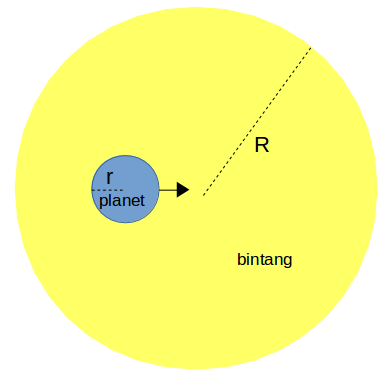
\includegraphics[scale=0.4]{transit-planet.png}
\caption{Planet transit di depan bintang induk.}
\end{figure}

Sebagian permukaan bintang tertutup oleh planet. Planet dianggap sebagai benda gelap yang tidak berkontribusi pada kecerlangan yang pengamat terima. Dengan demikian, berlaku:

\begin{eqnarray*}
m_{transit}-m_0 &=& -2,5\log \dfrac{E_{transit}}{E_0}\\
0,0128&=&  -2,5\log \dfrac{E_0-\frac{A_{planet}}{A_{bintang}}E_0}{E_0}\\
0,0128&=&  -2,5\log (1-\frac{A_{planet}}{A_{bintang}})\\
\log (1-\frac{A_{planet}}{A_{bintang}})&=&\frac{-0,0128}{2,5}\\
\log (1-\frac{\pi r^2}{\pi R^2})&=&\frac{-0,0128}{2,5}\\
1-\frac{\pi r^2}{\pi R^2}&=&0,98828\\
\frac{\pi r^2}{\pi R^2}&=&0,01172\\
r&=&0,11
\end{eqnarray*}
Jari-jari planet sekitar 0,11 kali jari-jari bintang induknya.\\


\question Setiap satu reaksi penggabungan nuklir di pusat Matahari melibatkan 6 proton yang akhirnya menghasilkan kembali 2 proton dan 1 inti helium ($^{4}_{2}$He). Dengan mengabaikan massa nukleon lain (misal positron), hitunglah besar energi per detik yang dihasilkan jika jumlah reaksi per detik sebanyak $10^{34}$.\\

Jawaban:

Energi yang dihasilkan berasal dari perubahan massa menjadi energi, dalam sekali reaksi $E = \Delta m . c^{2}$ dengan $\Delta m \cong (4 \times m_p) - (1 \times m_{\texttt{He}})$\\
massa proton $(m_p) = 1.67262178 \times 10^{-27}$ kg\\
massa inti He $(m_{\texttt{He}}) = 6.64465675 \times 10^{-27} $ kg\\
kecepatan cahaya $(c) = 299792458$ m/s\\   
$\Delta m = 4.583 \times 10^{-29}$ kg\\
$E = 4.119 \times 10^{-12}$ Joule\\
Jika terdapat $10^{34}$ reaksi tiap detik maka energi yang dihasilkan adalah $4.119 \times 10^{22}$ Joule.\\


\question Berdasarkan konfigurasi bintang ganda spektroskopi relatif terhadap pengamat yang sebidang dengan bidang orbit sistem bintang ganda, seperti di gambar bawah, buatlah kurva kecepatan radial (dalam km/s) terhadap fase orbit. Diketahui
\begin{choices}
\choice $M_1=1M_{\odot}$, $M_2=2M_{\odot}$
\choice Periode orbit, $P=30$ hari
\choice Kecepatan radial titik pusat massa, $v_{pm}=+42$ km/s
\end{choices}

\begin{figure}[H]
\centering
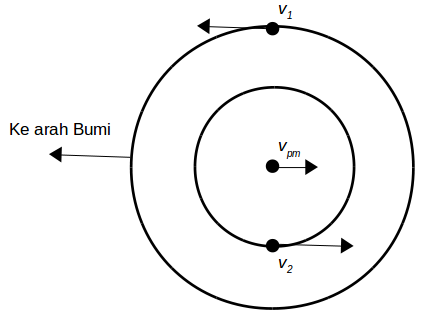
\includegraphics[scale=0.55]{bintang-ganda.png}
\caption{Sketsa bintang ganda.}
\end{figure}

Jawaban:
Mula-mula tentukan kecepatan orbit masing-masing bintang terhadap pusat massa, asumsi orbit lingkaran.

\begin{eqnarray}
M_1 r_1=M_2 r_2
\end{eqnarray}

Untuk $a$ dalam sa dan $P$ dalam tahun, berlaku:

\begin{eqnarray}
\dfrac{a^3}{P^2}=M_1+M_2
\end{eqnarray}

dengan $a=r_1+r_2$.

\begin{eqnarray*}
\dfrac{a^3}{P^2}&=&M_1+M_2\\
\dfrac{(r_1+r_2)^3}{P^2}&=&M_1+M_2\\
r_1+r_2&=&0,27 \text{  sa}\\
r_1+r_2&=&4,08\times10^7 \text{  km}
\end{eqnarray*}

Masukkan hasil tersebut ke persamaan (1), didapat:

$r_1=2,72\times10^7$ km

$r_1=1,36\times10^7$ km

sehingga didapati $v_1=\frac{2\pi r_1}{P}=65,910$ km/s dan $v_2=\frac{2\pi r_1}{P}=32,955$ km/s. Dengan bantuan gambar di atas, tampak bahwa kecepatan radial maksmimum dan minimum bintang pertama: $v_{1-max}=v_1+v_{pm}=107,910$ km/s dan $v_{1-min}=-v_1+v_{pm}= -23,910$ km/s, sedangkan untuk bintang kedua $v_{2-max}=v_2+v_{pm}=74,955$ km/s dan $v_{2-min}=-v_2+v_{pm}= 9,045$ km/s. Fase ditentukan dari $\frac{t}{P}$. Kurva kecepatan radial didapat sebagai berikut:

\begin{figure}[H]
\centering
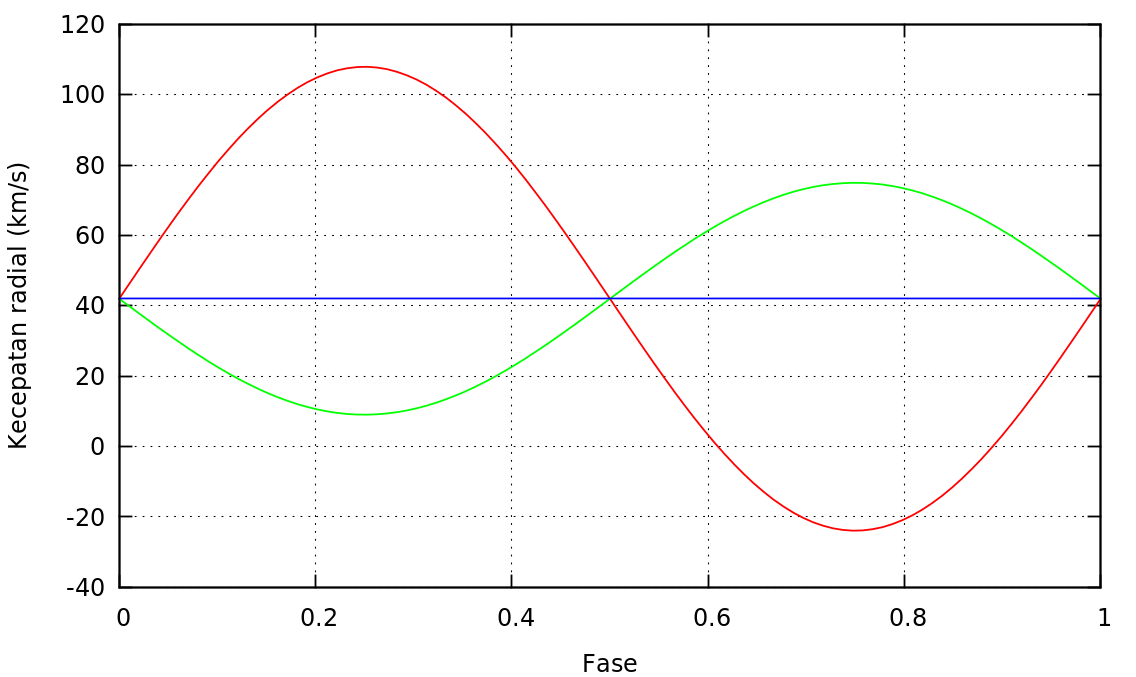
\includegraphics[width=0.55\textwidth]{kec-radial.png}
\caption{Kurva kecepatan radial bintang ganda, garis merah menyatakan kecepatan bintang pertama, garis hijau menyatakan bintang kedua.}
\end{figure}

\newpage
\textbf{Soal Essay Panjang}

\question Sebuah satelit geostationer yang massanya 800 kg mengelilingi Bumi dalam orbit lingkaran. Tiba-tiba satelit itu ditabrak oleh sebuah meteoroid kecil yang massanya 120 kg. Dilihat dari Bumi, meteoroid itu bergerak di bidang langit dengan kecepatan 4,2 km/s, dengan arah mirip gerak satelit tapi membentuk sudut kira-kira $30^{\circ}$ terhadap arah gerak satelit tersebut. Setelah tabrakan, meteoroid itu melesat ke dalam satelit tapi tidak menghancurkannya. Berapa kecepatan satelit sesaat setelah tumbukan dan kemana arahnya yang baru?\\


Jawaban: 

Hukum Kepler dapat diturunkan dari gerak melingkar dan gravitasi Newton. Asumsi orbit lingkaran dan $M >> m$
\begin{eqnarray*}
F_{s} &=& F_{g}\\
ma_s &=& \frac{GMm}{r^{2}}\\
\frac{v^2}{r} &=& \frac{GM}{r^{2}} \rightarrow v = \sqrt{\frac{GM}{r}}, v = \frac{2 \pi r}{P}\\
\frac{4 \pi^{2} r^{3}}{P^{2}} &=& GM 
\end{eqnarray*}
Satelit geostationer merupakan satelit dengan gerak searah rotasi Bumi dan periode sama dengan periode rotasi Bumi ($P = 23^{h}56^{m}$). Oleh karena itu akan diperoleh jarak satelit dari Bumi ($r$) $\cong 42164$ km\\

Kecepatan orbit satelit dapat dihitung dengan\\
$v = \sqrt{\frac{GM}{r}}$ atau $v = \frac{2 \pi r}{P}$\\
$v_s \cong 3.0746$ km/s

\begin{figure}[H]
\centering
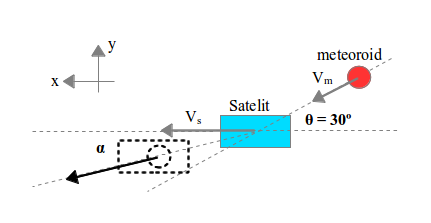
\includegraphics[width=0.49\textwidth]{satelit_meteoroid.png}
\caption{Skema tumbukan dimana kedua objek menyatu setelah terjadi tumbukan (tidak lenting sama sekali).}
\label{overflow}
\end{figure}

dengan skema tumbukan dan arah sumbu koordinat yang digunakan seperti di atas, maka dapat diuraikan:\\
$v_{sx} = v_s = 3.0746$ km/s\\
$v_{sy} = 0$ km/s\\
$v_{mx} = v_m \cos \theta = 3.6373$ km/s\\
$v_{my} = v_m \sin \theta = 2.1$ km/s arah $y$-neg\\

Hukum kekekalan momentum\\
Sumbu-$x$\\
$m_{s}v_{sx} + m_{m}v_{mx} = (m_{s} + m_{m})v_{x}$\\
$v_x = 3.148$ km/s\\

Sumbu-$y$\\
$m_{s}v_{sy} + m_{m}v_{my} = (m_{s} + m_{m})v_{y}$\\
$v_y = -0.274$ km/s\\

Sesaat setelah tumbukan kecepatan satelit $v = 3.148\hat{i} - 0.274\hat{j}$, sehingga besarnya $\Vert v \Vert = \sqrt{v_x^2 + v_y^2} = 3.16$ km/s. Arahnya dapat ditentukan dengan $\tan \alpha = \frac{v_y}{v_x}$, sehingga diperoleh satelit berbelok sebesar $ \alpha \cong 5^{\circ}$ ke arah gerak meteoroid.\\

\question Bintang Barnard adalah salah satu bintang dekat Matahari yang memiliki gerak diri terbesar ($\mu$=10,34"/tahun). Bintang tersebut memiliki kecepatan radial sebesar -108 km/s, dan paralaks sebesar 0,546". Suatu saat di masa depan, bintang tersebut akan berpapasan dekat dengan Matahari. Gambarkanlah komponen kecepatan bintang Barnard terhadap Matahari! Hitunglah jarak terdekat bintang Barnard terhadap Matahari dan kapan saat itu terjadi?

Jawaban:

Sketsa:

\begin{figure}[H]
\centering
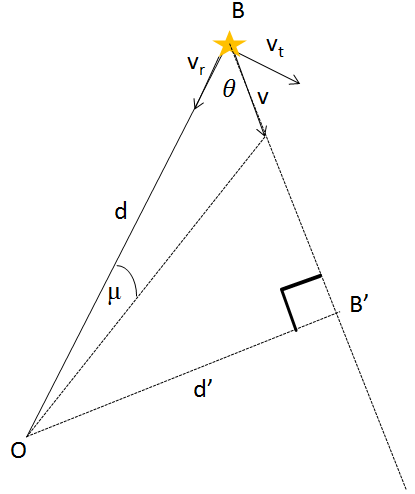
\includegraphics[scale=0.55]{barnard.png}
\caption{B menyatakan posisi bintang Barnard sekarang terhadap pengamat O di Matahari, $v$ menyatakan kecepatan ruang bintang Barnard, $d$ jaraknya sekarang dan $d'$ jarak terdekat bintang Barnard suatu hari nanti.}
\end{figure}

Dengan geometri seperti pada gambar, berlaku

\begin{eqnarray*}
\sin \theta=&\dfrac{d'}{d}=&\dfrac{v_t}{v}\\
&\dfrac{d'}{d}=&\dfrac{v_t}{\sqrt{v_r^2+v_t^2}}\\
&\dfrac{d'}{d}=&\dfrac{4,74\mu d}{\sqrt{v_r^2+(4,74\mu d)^2}}\\
&\dfrac{d'}{d}=&\dfrac{4,74\frac{\mu}{p}}{\sqrt{v_r^2+(4,74\frac{\mu}{p})^2}}\\
&d'=&1,17 pc\\
\\
&t=&\dfrac{d\cos \theta}{v}\\
&t=&9,81\times10^3 \text{  tahun}
\end{eqnarray*}

Jarak terdekat bintang Barnard 1,17 pc dan jarak ini akan dicapai $9,81\times10^3$ tahun kemudian.\\


\question Dua buah gugus bintang, A dan B, yang terletak pada arah bujur galaksi $l = 30^{\circ}$ memiliki kesamaan dalam jumlah bintang anggota, bentuk diagram Hertzsprung-Russel (HR), dan sebaran kecepatan. Gugus A tampak berdiameter $1^{\circ}$, berjarak 150 parsek, dan magnitudo semu bintang deret utama di titik belok diagram HR adalah $m_v = $3,56. Gugus B tampak berdiameter $6'$ dan magnitudo semu bintang deret utama di titik belok adalah $m_v = $10,18. Hitung berapa absorpsi antar bintang pada arah $l = 30^{\circ}$ dalam satuan magnitudo per kiloparsek!

Jawaban:

Keterangan yang diberikan menjurus pada asumsi atau kesimpulan bahwa gugus A dan B adalah dua gugus identik dengan diameter yang sama $D_{A} = D_{B}$. Sehingga jika $d_{A} = 150$ parsek, maka $d_{B} = \frac{60'}{6'} \times d_{A} = 1500$ parsek.\\ 
Dua bintang yang dibandingkan dapat diasumsikan pula sebagai dua bintang identik ($L_1 = L_2$ atau $M_1 = M_2$).
\begin{eqnarray*}
m_1 - M_1 &=& -5 + 5 \log d_A + kd_A\\
m_2 - M_2 &=& -5 + 5 \log d_B + kd_B\\
m_1 + 5 - 5 \log d_A - kd_A &=& m_2 + 5 - 5 \log d_B - kd_B\\
m_1 - 5 \log d_A - kd_A &=& m_2 - 5 \log d_B - kd_B\\
k(d_B - d_A) &=& m_2 - m_1 + 5 \log (d_A/d_B)\\
k &=& \frac{10.18 - 3.56 + 5 \log (150/1500)}{1500-150}\\
k &=& 0.0012
\end{eqnarray*}
diperoleh absorpsi antar bintang $k = 0.0012$ mag/pc = 1.2 mag/kpc \\


\question Diketahui periode rotasi Matahari di ekuatornya saat ini adalah 25 hari. Asumsikan massa Matahari kekal selama evolusinya. Jika Matahari berevolusi hingga akhirnya menjadi Katai Putih dengan kerapatan massa $2,51\times 10^9$ kg/m$^3$,
\begin{choices}
\choice hitunglah jejari dan periode rotasi Katai Putih!
\choice bagi planet-planet di Tata Surya, apakah akan mengalami perubahan pada periode dan ukuran orbitnya? Jelaskan!
\end{choices}

Jawaban:

\begin{choices}
\choice Dengan massa tetap, $M_{\odot}=4\pi r^3 \rho$, $r=5750,39$ km.

$M_{\odot}=2\times10^{30} $ kg

$R_{\odot}=696000 $ km

Asumsikan Matahari dan katai putih yang terbentuk nantinya merupakan benda pejal. Periode rotasi dihitung menggunakan prinsip kekekalan momentum sudut $L=I\omega=konstan$, sehingga berlaku:

\begin{eqnarray*}
(I\omega)_{awal}&=&(I\omega)_{akhir}\\
\dfrac{2}{5}M_{\odot}R_{\odot}^2\dfrac{2\pi}{P_{\odot}}&=&\dfrac{2}{5}M_{\odot}r^2\dfrac{2\pi}{P_{katai}}\\
P_{katai}&=&(\dfrac{r}{R_{\odot}})^2P_{\odot}\\
&=& 0,0017 \text{  hari}\\
&\approx& 2,5 \text{  menit}
\end{eqnarray*}

\choice Radius maupun periode orbit planet-planet di Tata Surya tidak akan berubah karena besaran-besaran tersebut hanya bergantung pada massa Matahari (sebagai massa yang sangat dominan di Tata Surya). Massa Matahari tidak berubah, energi total sistem tetap, maka radius orbit dan periode planet-planet akan tetap.\\
\end{choices}


\question Apabila garam dipanaskan, cahaya kuning yang terdiri atas dua garis emisi yang terpisah cukup dekat, yakni pada panjang gelombang 588,997 nm dan 589,594 nm akan dipancarkan. Garis-garis ini disebut garis Natrium D (\textit{Sodium D lines}) dan diamati oleh Fraunhofer dalam spektrum Matahari. Apabila cahaya ini jatuh pada sebuah kisi difraksi dengan 300 baris per milimeter, maka berapakah sudut antara spektrum orde kedua dari kedua panjang gelombang ini? Agar kedua garis emisi dapat dipisahkan, berapa baris per milimeter kisi yang diperlukan? (Diketahui 1 nm $= 10^{-9}$ m)\\

Jawaban:

\textit{Grating} ($N$) = 300 baris/mm\\
Jarak antar ``grate'' atau konstanta kisi ($d$)= 1/300 mm\\
Pola terang untuk kisi difraksi mengikuti persamaan 
\begin{equation*}
d \sin \theta = n \lambda 
\end{equation*}
dengan $n = 1, 2, 3, ...$\\

Dapat dihitung untuk orde-2 ($n=2$) sudut yang dibentuk terhadap arah sinar datang untuk masing-masing panjang gelombang adalah\\
$\theta_1 = 20.6953056549^{\circ}$\\
$\theta_2 = 20.7172462492^{\circ}$\\
sehingga $\Delta \theta = 0.0219405943^{\circ}$
 
Untuk dua panjang gelombang yang hampir sama besarnya, $\lambda_1$ dan $\lambda_2$, dimana kisi difraksi hampir tidak dapat memisahkannya, didefinisikan \textit{resolving power} (kemampuan memisahkan) dari kisi difraksi sebagai:
\begin{equation*}
R = \frac{\lambda}{\lambda_2 - \lambda_1} = \frac{\lambda}{\Delta \lambda}
\end{equation*}
semakin besar resolusi kisi difraksi artinya semakin kecil dua panjang gelombang yang dapat dipisahkan.

Resolusi kisi difraksi untuk orde difraksi ke-$m$ adalah 
\begin{equation*}
R = Nm
\end{equation*}
Semakin besar \textit{grating} dari kisi difraksi yang tersinari dan orde difraksi berarti semakin besar pula resolusinya.

Dapat diambil $\lambda$ rerata sebagai acuan yaitu $589.2955$ nm, dan $\Delta \lambda = 0.597$ nm.
\begin{equation*}
R = \frac{\lambda}{\Delta \lambda} = \frac{589.2955}{0.597} = 987.1
\end{equation*}
sehingga jumlah minimal garis yang disinari agar dapat memisahkan dua panjang gelombang di atas pada orde difraksi ke-2 adalah $N = R/m = 493.55 \cong 494$ baris. Dalam soal tidak diketahui lebar cahaya dan/atau lebar kisi, maka dengan asumsi lebar cahaya yang diterima kisi difraksi adalah 1 mm, maka butuh kisi difraksi dengan \textit{grating} 494 baris/mm.

\end{questions}

\end{document}
